\documentclass{article}

\usepackage[a4paper, total={7.0in, 10.0in}]{geometry}

\usepackage[pdftex]{graphicx}
\usepackage[czech]{babel}
\usepackage[utf8]{inputenc}
\usepackage{enumitem}
\setlist{leftmargin=4.8mm}
\usepackage{amsmath}
\usepackage{url}
\usepackage{listings}
\usepackage{caption}
\usepackage{gensymb}
\usepackage[usenames,dvipsnames,svgnames,table]{xcolor}
\usepackage{pdflscape}

\usepackage[pdftex]{hyperref}
\hypersetup{colorlinks=true,
  unicode=true,
  linkcolor=black,
  citecolor=black,
  urlcolor=black,
  bookmarksopen=true}

\usepackage{xcolor}
\colorlet{mygray}{black!30}
\colorlet{mygreen}{green!60!blue}
\colorlet{mymauve}{red!60!blue}
\lstset{
	backgroundcolor=\color{gray!10},  
	basicstyle=\ttfamily,
	columns=fullflexible,
	breakatwhitespace=false,      
	breaklines=true,                
	captionpos=b,                    
	commentstyle=\color{mygreen}, 
	extendedchars=true,              
	frame=single,                   
	keepspaces=true,             
	keywordstyle=\color{blue},      
	language=c++,                 
	numbers=none,                
	numbersep=5pt,                   
	numberstyle=\tiny\color{blue}, 
	rulecolor=\color{mygray},        
	showspaces=false,               
	showtabs=false,                 
	stepnumber=5,                  
	stringstyle=\color{mymauve},    
	tabsize=3,                      
	title=\lstname                
}

\usepackage{amssymb}
\renewcommand{\labelitemi}{{\textcolor{favyellow}{$\blacktriangleright$}}}

\usepackage[numbers,sort&compress]{natbib}
\usepackage{tgadventor}
\usepackage[explicit]{titlesec}
\usepackage{tikz}
\usepackage{tabularx}
\usepackage{fontawesome5}

\newcolumntype{Y}{>{\centering\arraybackslash}X}

\newcommand*\justify{
  \fontdimen2\font=0.4em
  \fontdimen3\font=0.2em
  \fontdimen4\font=0.1em
  \fontdimen7\font=0.1em
  \hyphenchar\font=`\-
}

\makeatletter
\def\subtitle#1{\gdef\@subtitle{#1}}
\def\maketitle{\begin{titlepage}%
		\let\footnotesize\small
		\let\footnoterule\relax
		\let \footnote \thanks
		\null\vfil
  \begin{figure}
    \centering
    
\includegraphics[width=\linewidth]{img/fav_kiv_cmyk.pdf}
  \end{figure}
		\vskip 140\p@
		\begin{center}%
			{\fontsize{32}{32}\fontfamily{qag}\selectfont \@title \par}%
			\vskip 2.5em% Added this
			{\fontsize{18}{18}\fontfamily{qag}\selectfont \@subtitle \par}% and this
			\vspace{\fill}
		\end{center}\par
        {\fontsize{12}{12}\fontfamily{qag}\selectfont Autor: \@author \par}
        {\fontsize{12}{12}\fontfamily{qag}\selectfont Revize: 2.1 (1. 9. 2025) \par}
		\@thanks
		\vfil\null
	\end{titlepage}%
	\setcounter{footnote}{0}%
	\global\let\thanks\relax
	\global\let\maketitle\relax
	\global\let\@thanks\@empty
	\global\let\@author\@empty
	\global\let\@date\@empty
	\global\let\@title\@empty
	\global\let\title\relax
	\global\let\author\relax
	\global\let\date\relax
	\global\let\and\relax
}
\makeatother

\setlength{\parskip}{4pt}

% NASTAVENI JAZYKA: #1 pro CZ, #2 pro EN
\newcommand\lang[2]{#1}

\title{KIV-DPP-02}
\subtitle{\lang{Dokumentace rozšiřující desky}{Expansion board documentation}}
\author{Martin Úbl}
\date{\lang{1. září 2025}{1 September 2025}}

\begin{document}

\maketitle
\definecolor{favyellow}{RGB}{218,169,71}

%\titleformat{\section}
%  {\normalfont\sffamily\Large\bfseries\color{favyellow}}
%  {\thesection}{1em}{}

\titleformat{\section}
    [hang]
    {\Large\bfseries}
    {}
    {0pt}
    {\tikz{
    \node[draw, rounded corners=1mm,text depth=0.2ex,line width=2pt,anchor=west,color=favyellow](a){\fontsize{18}{18}\selectfont\normalfont\sffamily\bfseries\textcolor{favyellow}{}#1};
    \coordinate (b) at (\textwidth,0);
    \draw[line width=2pt,color=favyellow] (a)--(b);}}

\titleformat{\subsection}
    [hang]
    {\Large\bfseries}
    {}
    {0pt}
    {\tikz{
    \node[draw, rounded corners=1mm,text depth=0.2ex,line width=1pt,anchor=west,color=favyellow](a){\fontsize{14}{14}\selectfont\normalfont\sffamily\bfseries\textcolor{favyellow}{}#1};
    \coordinate (b) at (\textwidth,0);
    \draw[line width=1pt,color=favyellow] (a)--(b);}}


\section{\lang{Přehled periferií}{Board overview}}

\begin{figure}[ht]
	\centering
	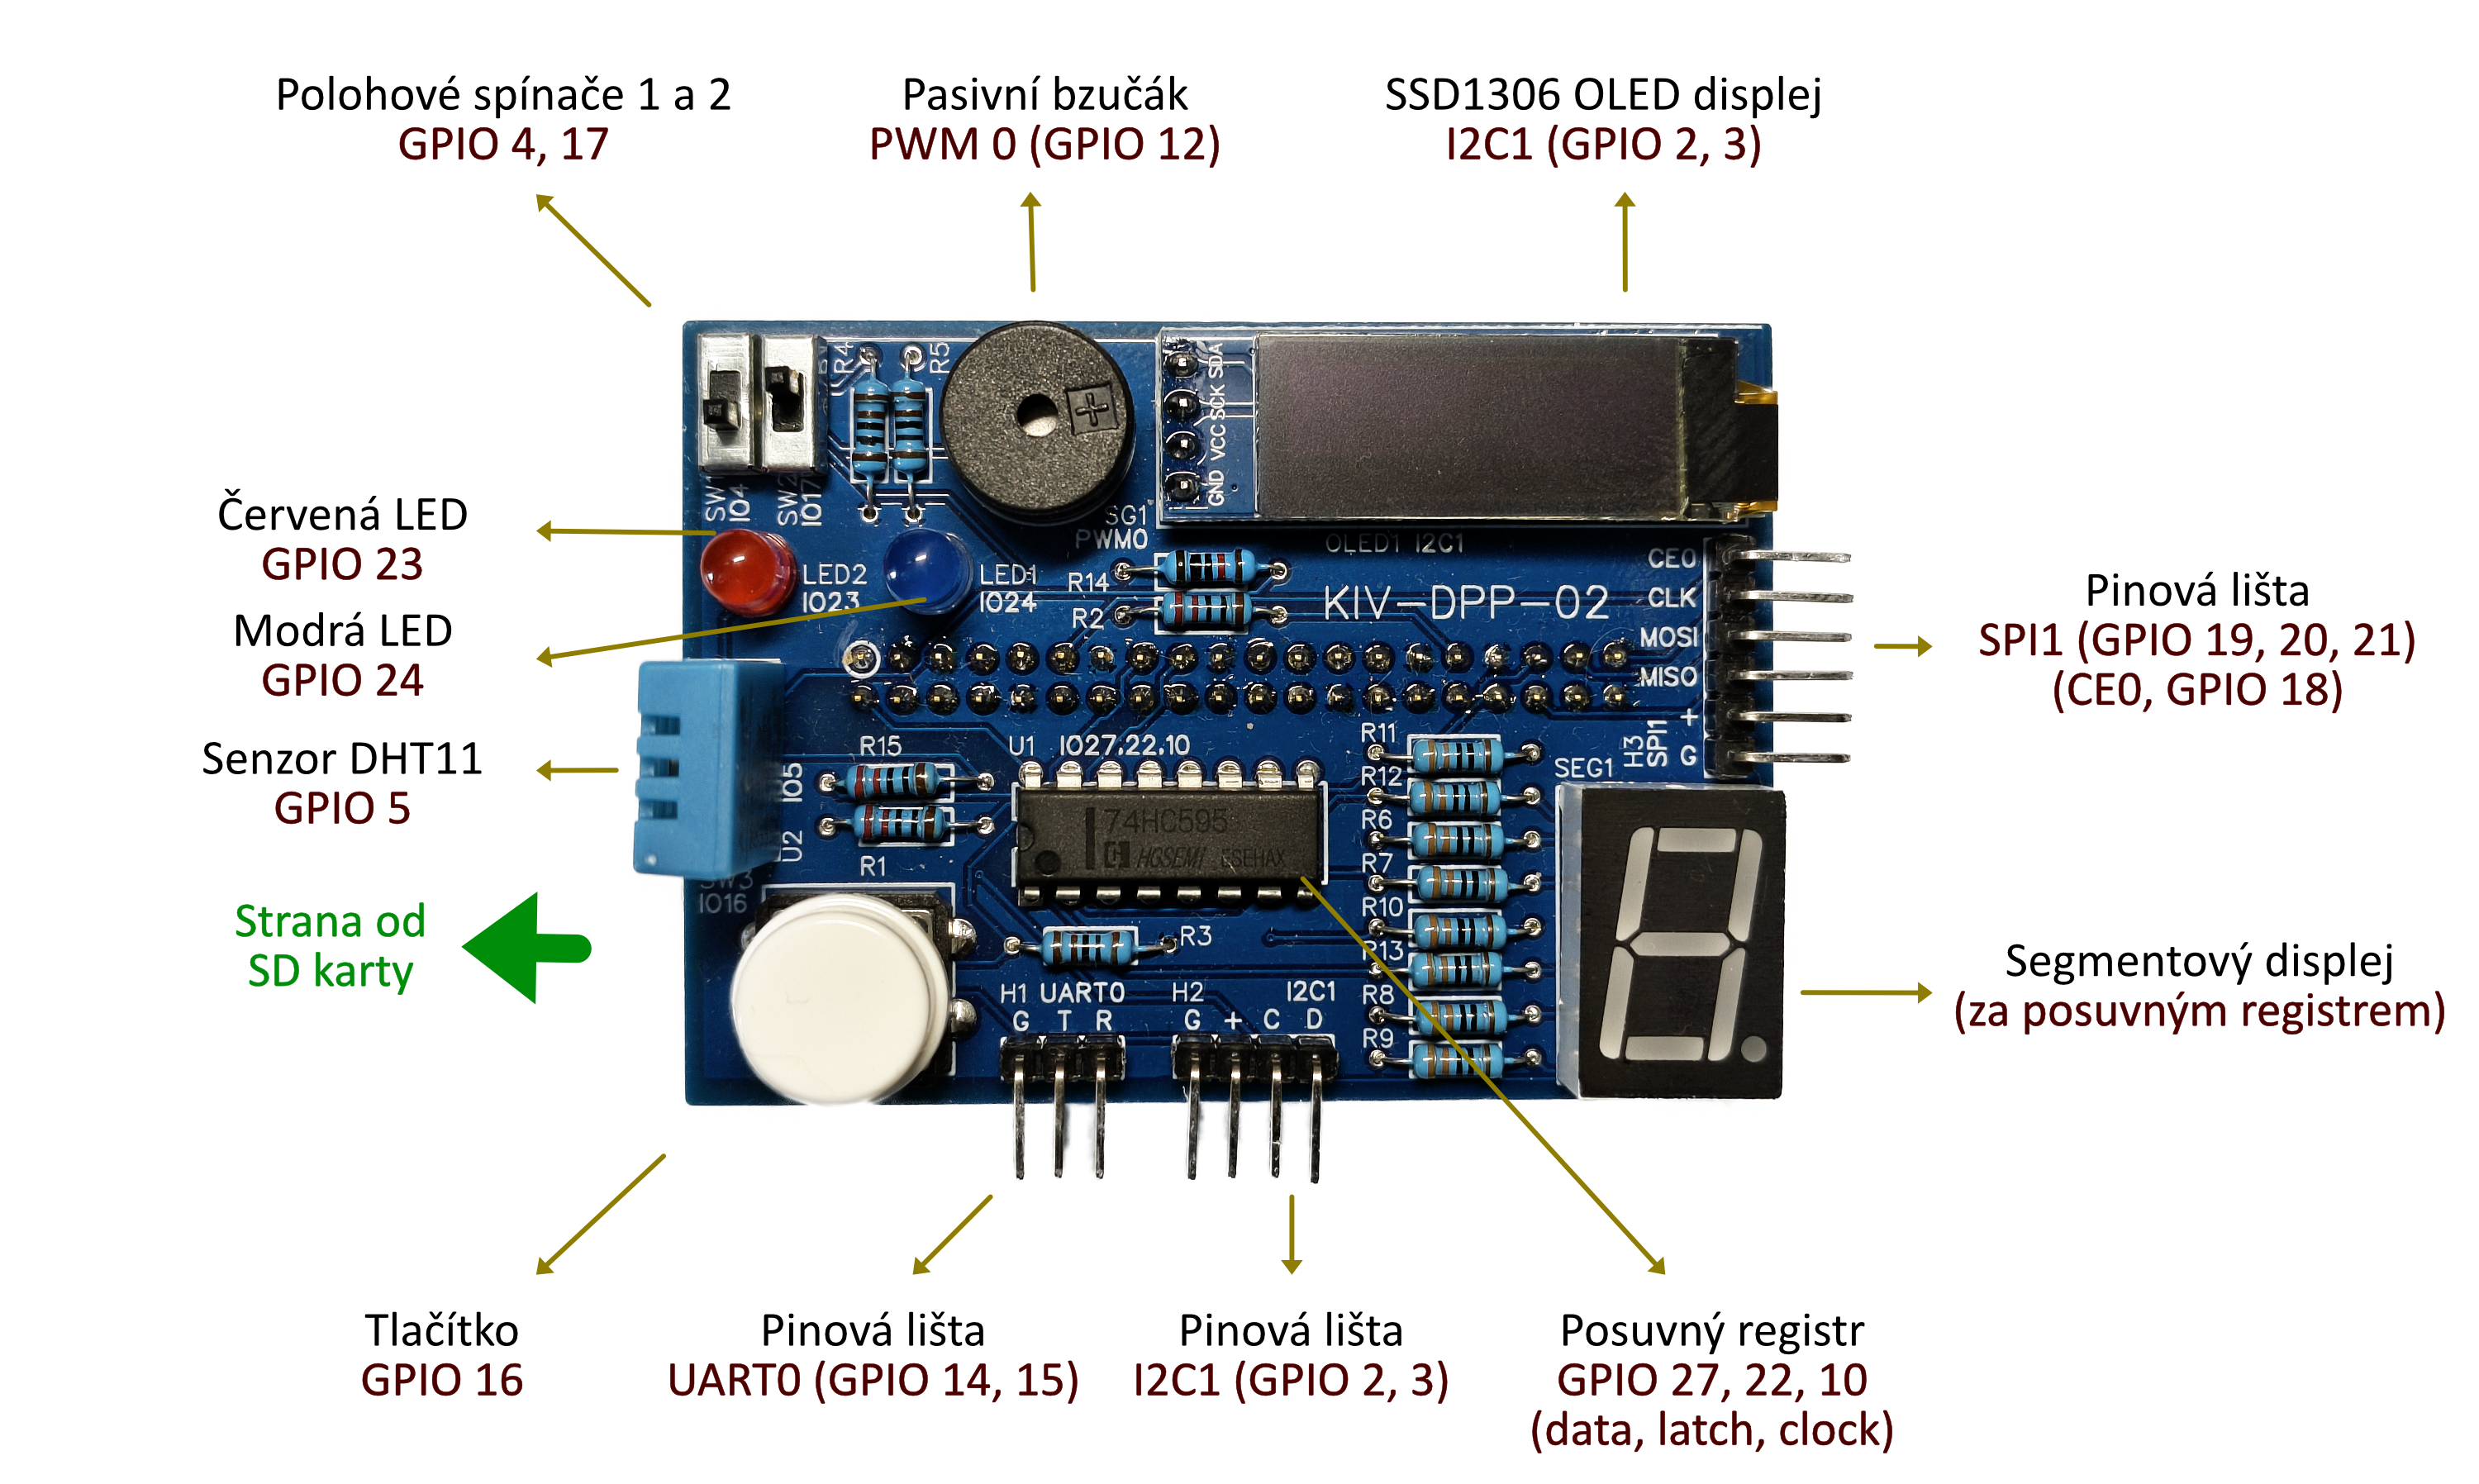
\includegraphics[width=1.0\linewidth]{img/kiv-dpp-02-front.png}
\end{figure}

\vspace{5em}

\noindent
\bgroup
\def\arraystretch{1.5}
\begin{tabularx}{\textwidth}{X|c|c|l}
            \cellcolor{favyellow!25}\textbf{\lang{Periferie/modul}{Peripheral/module}} &
            \cellcolor{favyellow!25}\textbf{\lang{Rozhraní/kanál}{Interface/channel}} &
            \cellcolor{favyellow!25}\textbf{GPIO} &
            \cellcolor{favyellow!25}\textbf{\lang{Poznámka}{Note}}
            \\\hline
        \lang{Červená}{Red} LED & -- & 23 & \\\hline 
        \lang{Modrá}{Blue} LED & -- & 24 & \\\hline
        \lang{Senzor teploty a vlhkosti}{Temperature and humidity sensor} DHT11 & -- & 5 & \\\hline
        \lang{Tlačítko}{Push button} & -- & 16 & \\\hline
        UART header & UART0 & 14, 15 & \\\hline
        I2C header & I2C1 & 2, 3 & \\\hline
        SPI header & SPI1 & 19, 20, 21 & CE0 (GPIO 18) \\\hline
        \lang{Posuvný registr}{Shift register} 74HC595 & -- & 27, 22, 10 & data, latch, clock \\\hline
        \lang{Sedmi-segmentový displej}{7-segment display} & -- & -- & \lang{přímo připojen na posuvný registr}{directly connected to the shift register} \\\hline
        SSD1306 OLED \lang{displej}{display} & I2C1 & 2, 3 & 128x32 \lang{bodů}{pixels}\\\hline
        \lang{Pasivní bzučák}{Passive buzzer} & PWM0 & 12 & \\\hline
        \lang{Polohový přepínač}{Switch} 1 & -- & 4 & \\\hline
        \lang{Polohový přepínač}{Switch} 3 & -- & 17 & \\\hline
\end{tabularx}
\egroup

\newpage\thispagestyle{empty}\setlength{\parskip}{0pt}
\begin{landscape}
\section*{\lang{Schéma desky}{Board schematic}}
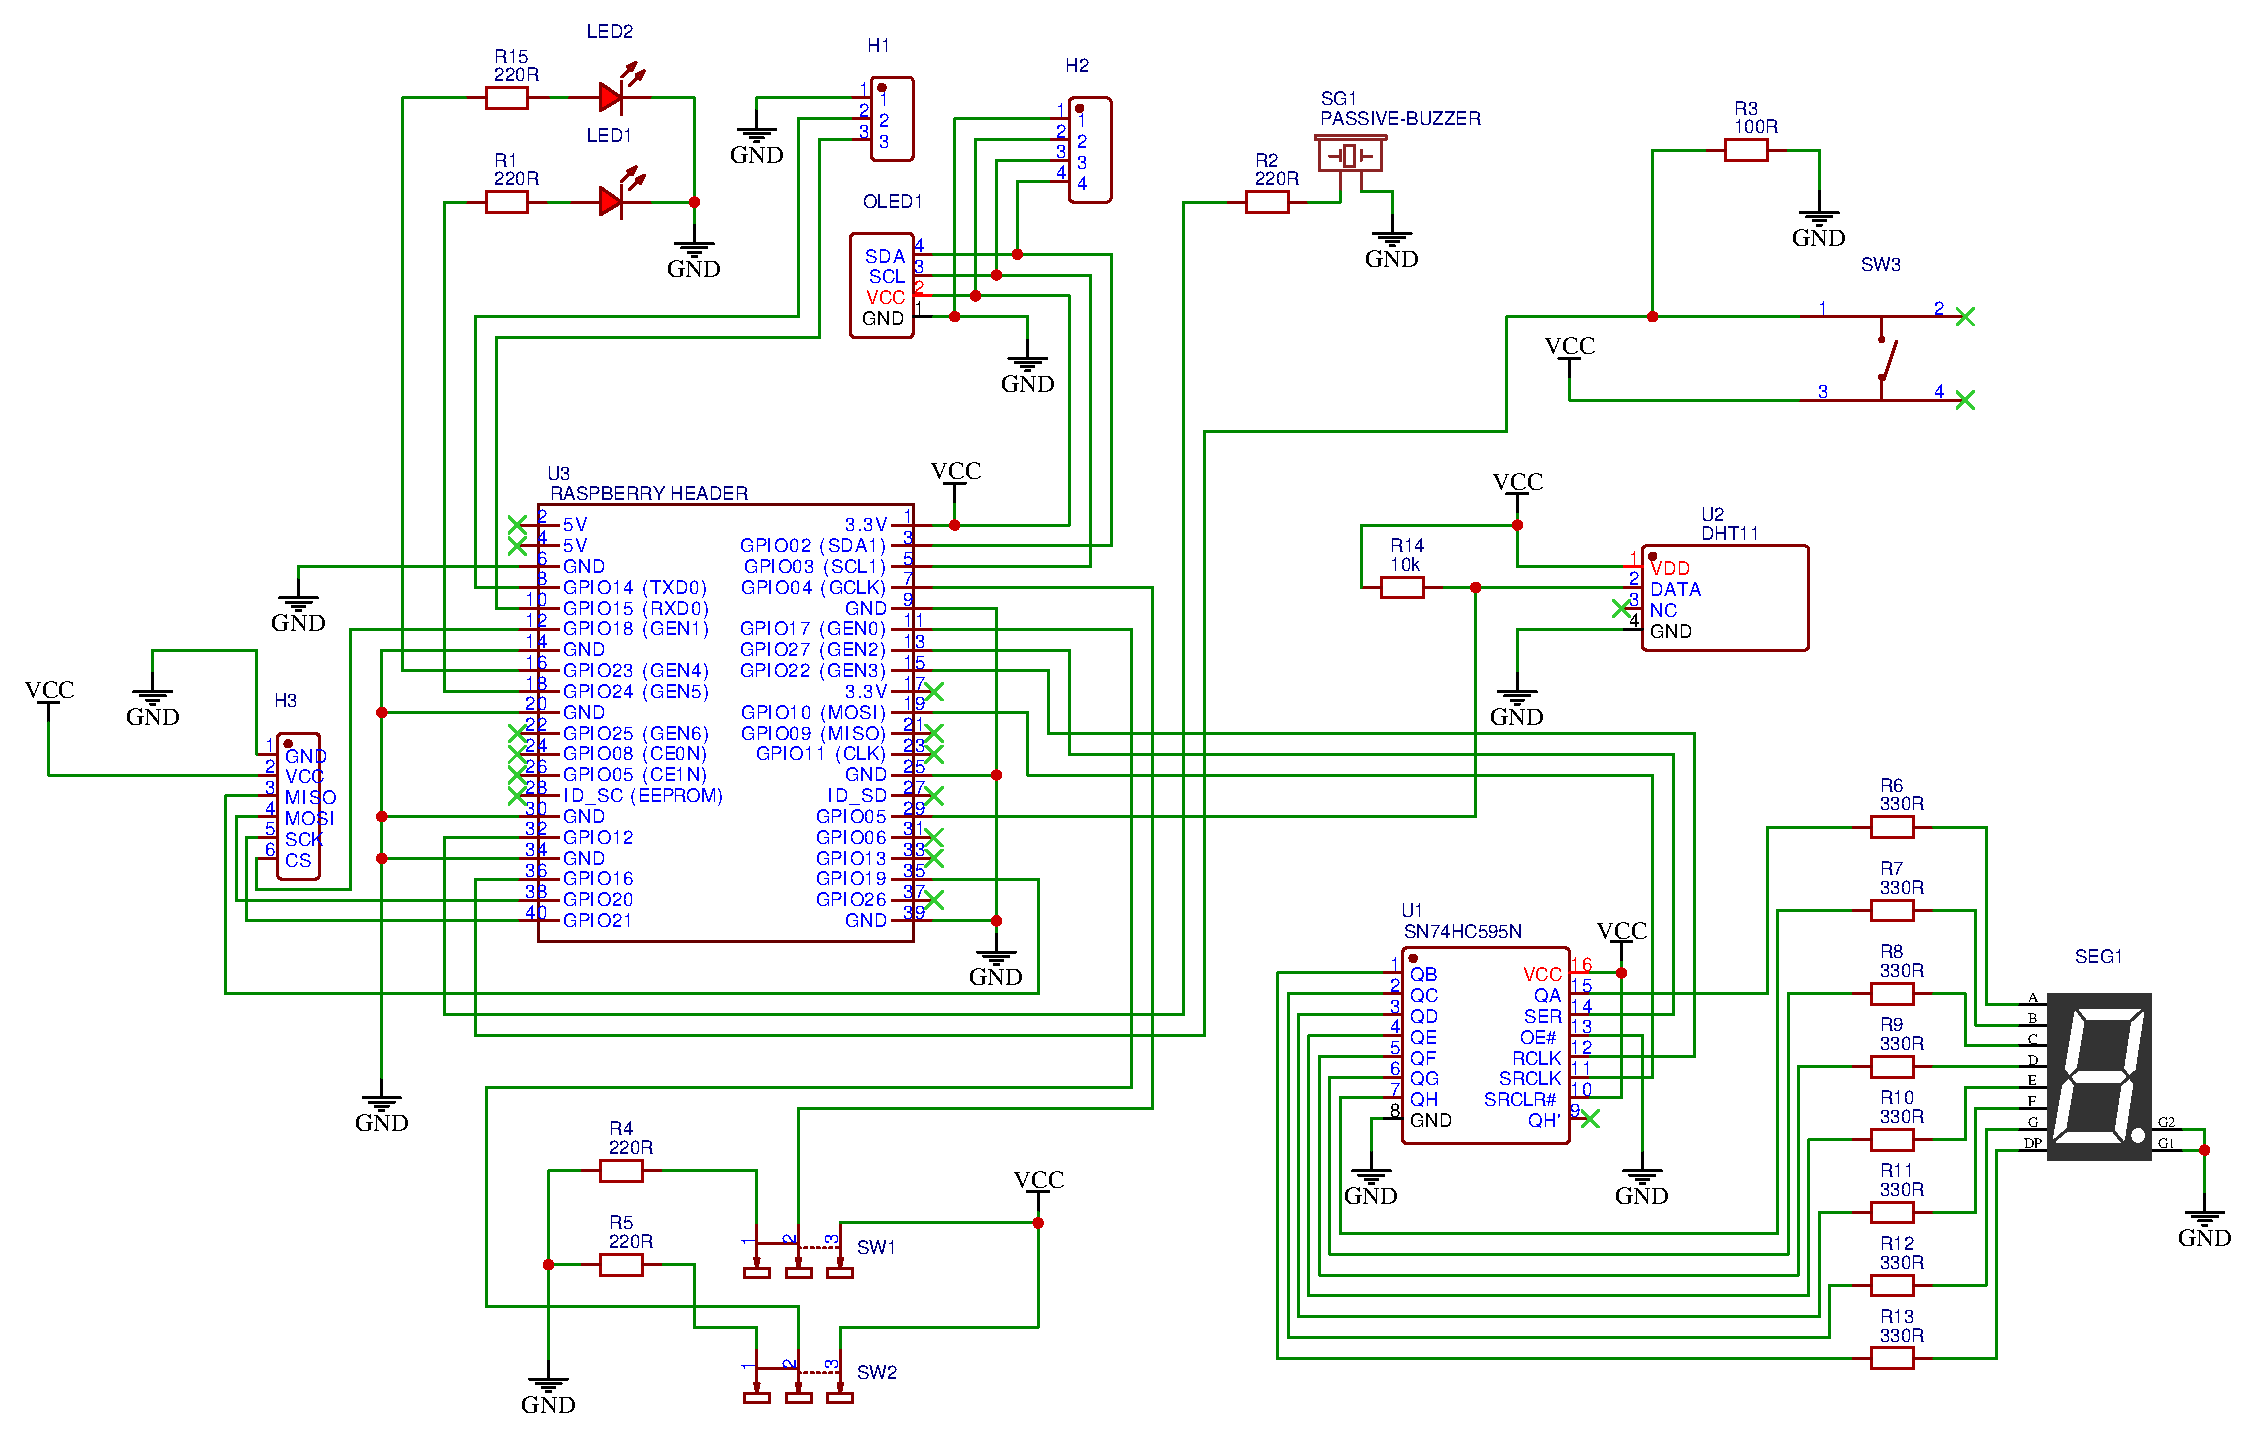
\includegraphics[width=\linewidth]{img/kiv-dpp-02-schema.pdf}
\end{landscape}
\newpage

\section{\lang{Zapojení}{Connection}}
\setlength{\parskip}{4pt}
\lang{Deska obsahuje 40-pinový header (2x20), který přímo pasuje do pinového protikusu na straně Raspberry Pi. Důležité je dodržet orientaci rozšiřující desky vůči Raspberry Pi -- v případě připojení na Raspberry Pi Zero, musí být DHT11 a LED na rozšiřující desce na straně, kde se na hostitelské desce nachází slot na SD kartu. Segmentový displej se pak nachází na straně, kde má hostitelská deska umístěné USB konektory.
}
{
The board contains a 40-pin F header, which is intended to be directly connected to M header on the Raspberry Pi side. It is important to rotate the board correctly -- in case of Raspberry Pi Zero, the DHT11 sensor and LEDs on the expansion board must be on the same side, as the SD card slot on the host board. The segment display is then localized on the same side, as USB ports on the host board.
}

\noindent
\lang{Dolní strana desky obsahuje vodicí značky, šipkami je označená strana SD karty a strana USB konektorů. \textbf{Vždy se při připojování přesvědčte, že desku zapojujete ve správné orientaci! Nesprávné připojení může vést ke zničení elektroniky rozšiřující i hostitelské desky.}}{The bottom side of the expansion board contains markers -- arrows pointing at the SD card side and USB side. \textbf{Always make sure, that you are connecting the expansion board the right way! Incorrect connection may lead to the destruction of electronics of the expansion or host board.}}

\section{\lang{Periferie a moduly}{Peripherals and modules}}

\subsection{LED 1, 2}

\begin{itemize}[nosep]
	\item \lang{\textbf{Barva}: červená, modrá}{\textbf{Color}: red, blue}
	\item \textbf{GPIO}: 23 \lang{(červená)}{(red)}, 24 \lang{(modrá)}{(blue)}
	\item \textbf{\lang{Spotřeba}{Current}}: max. 20 mA
	\item \textbf{\lang{Svítivost}{Luminosity}}: max. 3000 mcd
\end{itemize}

\vspace{1em}

\noindent
\lang{Klasická červená a modrá LED, anoda je vyvedená na GPIO pin 23 (červená) a 24 (modrá), katoda na GND.}{Standard red and blue LED, anode is connected to GPIO pin 23 (red) and 24 (blue), cathode is connected to GND.}

\subsection{\lang{Pasivní bzučák}{Passive buzzer}}

\begin{itemize}[nosep]
	\item \textbf{GPIO}: 12
    \item \textbf{\lang{PWM kanál}{PWM channel}}: 0
	\item \textbf{\lang{Odpor}{Resistance}}: 16 $\Omega$
\end{itemize}

\vspace{1em}

\noindent
\lang{Pasivní bzučák zapojený na GPIO 12 (PWM kanál 0). Bzučák je pasivní, takže nemá interní oscilátor -- je nutné ho tedy řídit PWM signálem.}{Passive buzzer connected to GPIO 12 (PWM channel 0). The buzzer is passive, so it does not have the internal oscilator -- the pulse-width modulation (PWM) is needed to drive the buzzer.}

\subsection{\lang{Tlačítko}{Push button}}

\begin{itemize}[nosep]
	\item \textbf{GPIO}: 16
	\item \lang{\textbf{Zapojení}: pull-up}{\textbf{Wiring}: pull-up}
\end{itemize}

\vspace{1em}

\noindent
\lang{Klasické tlačítko s plastovou čepičkou. Tlačítko není vybavenou debouncing obvodem, kompenzaci je tedy nutné provést softwarově.}{Standard push button with plastic cap. The button does not have a debouncing electronics bundled in, so the compensation must be done in software.}

\subsection{\lang{Polohový přepínač 1, 2}{Switches 1, 2}}

\begin{itemize}[nosep]
	\item \textbf{GPIO}: 4 (\lang{SW1, vlevo}{SW1, left}), 17 (\lang{SW2, vpravo}{SW2, right})
\end{itemize}

\vspace{1em}

\noindent
\lang{Běžné malé nezávisle zapojené polohové přepínače.}{Common switches, connected independently.}

\subsection{\lang{Posuvný registr}{Shift register}}

\begin{itemize}[nosep]
	\item \textbf{GPIO}: 27 (data), 22 (latch), 10 (clock)
	\item \textbf{Datasheet}: \url{http://home.zcu.cz/~ublm/files/os/74HC565.pdf}
\end{itemize}

\vspace{1em}

\noindent
\lang{Posuvný registr 74HC595N je vstupy zapojen přímo na GPIO 27 (datový pin), 22 (latch pin, přepnutí banku) a 10 (časovací signál). Výstupy jsou zapojeny na vstupy sedmi-segmentového displeje.}{The shift register 74HC595N is connected to GPIO 27 (data pin), 22 (latch pin, bank shift) and 10 (timing signal). Outputs are connected to inputs of the 7-segment display.}

\subsection{\lang{Sedmi-segmentový displej}{7-segment display}}

\begin{itemize}[nosep]
	\item \lang{\textbf{Zapojení}: společná katoda}{\textbf{Wiring}: common cathode}
    \item \textbf{\lang{Předřazený modul}{Preceding module}}: \lang{posuvný registr}{shift register}
	\item \textbf{\lang{Spotřeba}{Current}}: max. 15 mA
	\item \textbf{Datasheet}: \url{http://home.zcu.cz/~ublm/files/os/5161AS.pdf}
\end{itemize}

\vspace{1em}

\noindent
\lang{Sedmi-segmentový displej 5161AS je připojený na výstupy posuvného registru. Nelze jej tedy ovládat samostatně. Zapojení je se společnou katodou.}{7-segment display 5161AS is connected directly to the outputs of the shift register. It's not possible to control it directly. It is wired with common cathode.}

\noindent
\lang{Zobrazovací jednotka je na výstupy posuvného registru připojena následovně:}{The display is connected to the shift register as follows:}
\begin{figure}[ht!]
	\centering
	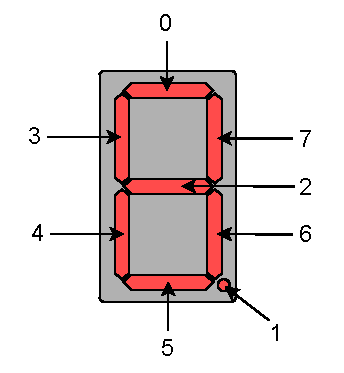
\includegraphics[width=0.3\linewidth]{img/kiv-dpp-02-segments.pdf}
\end{figure}

\noindent
\lang{Čísla představují pořadové číslo bitu do registru nahraného. Číslo 0 je tedy nejnovější nahraný bit, číslo 7 nejstarší.}{The numbers denote the ordinal number of bit shifted into the register. Number 0 is the latest shifted bit, number 7 is the oldest one.}

\subsection{OLED \lang{displej}{display}}

\begin{itemize}[nosep]
	\item \textbf{GPIO}: 2 (SDA), 3 (SCL)
	\item \lang{\textbf{Zapojení}: I2C kanál 1}{\textbf{Wiring}: I2C channel 1}
	\item \lang{\textbf{Typ}: monochromatický (modrá nebo bílá)}{\textbf{Type}: monochromatic (blue or white)}
	\item \lang{\textbf{Velikost matice}: 128x32 bodů}{\textbf{Matrix size}: 128x32 pixels}
    \item \lang{\textbf{I2C adresa}}{\textbf{I2C address}}: \texttt{0x3C}
	\item \textbf{Datasheet}: \url{http://home.zcu.cz/~ublm/files/os/SSD1306.pdf}
\end{itemize}

\vspace{1em}

\noindent
\lang{Displej SSD1306 je přímo připojený na piny 2 a 3, na kterých na hostitelské desce operuje I2C kanál 1. Protokol pro ovládání displeje je shodný pro všechny displeje s řadičem SSD1306 (všechny rozměry). Body displeje mohou svítit buď bílou nebo modrou barvou.}
{The SSD1306 display is directly connected to pins 2 and 3, on which the host board operates I2C channel 1. The protocol is common for all SSD1306-driven displays (all variants and dimensions). Pixels glow either blue or white.}

\noindent
\lang{Kanál I2C 1 je sdílený s kanálem vyvedeným na pinovou lištu. Adresa displeje osazeného na desce je \texttt{0x3C}.}{The I2C channel 1 is shared with the pin header mounted on board. The address of the display on the board is \texttt{0x3C}.}

\subsection{UART header}

\begin{itemize}[nosep]
	\item \textbf{GPIO}: 14 (TXD), 15 (RXD)
\end{itemize}

\vspace{1em}

\noindent
\lang{Header pro připojení UART terminálu, např. USB-TTL převodníku do hostitelského PC. Zapojení pinů je přímé -- do hostitelského počítače tedy musí být překřížené (RXD na straně desky je TXD na straně hostitele a naopak).}
{Header for UART terminal connection, e.g. the USB-TTL converter to host PC. The wiring is direct -- wiring should be crossed over to the other end (RXD on the board side to the TXD on the host side and vice versa).}

\subsection{I2C header}

\begin{itemize}[nosep]
	\item \textbf{GPIO}: 2, 3
    \item \textbf{\lang{I2C kanál}{I2C channel}}: 1
\end{itemize}

\vspace{1em}

\noindent
\lang{Header pro připojení I2C periferií na kanálu 1. Kanál je sdílený s OLED displejem.}
{Header for connecting I2C peripherals on channel 1. The channel is shared with the OLED display.}

\subsection{SPI header}

\begin{itemize}[nosep]
	\item \textbf{GPIO}: 19, 20, 21, 18
    \item \textbf{\lang{SPI kanál}{SPI channel}}: 1
\end{itemize}

\vspace{1em}

\noindent
\lang{Header pro připojení SPI periferií na kanálu 1. Do lišty je vyveden i hardwarový chip select CE0 na GPIO pinu 18.}
{Header for connecting SPI peripherals on channel 1. The header contains hardware chip select signal CE0 on GPIO 18.}

\subsection{\lang{Senzor teploty a vlhkosti DHT11}{Temperature and humidity sensor DHT11}}

\begin{itemize}[nosep]
	\item \textbf{GPIO}: 5
	\item \textbf{Datasheet}: \url{http://home.zcu.cz/~ublm/files/os/dht11.pdf}
\end{itemize}

\vspace{1em}

\noindent
\lang{Senzor teploty a vlhkosti DHT11 připojený na GPIO 5. Komunikuje pomocí rozhraní 1-Wire, které nemá v Raspberry Pi Zero hardwarovou podporu.}
{Temperature and humidity sensor DHT11 connected to GPIO 5. It communicates using the 1-Wire protocol, which does not have a built-in hardware support in Raspberry Pi Zero.}


\newpage

\section{Revize}

\subsection{2.0}

Úvodní sestavení dokumentu, revize desky, výroba, pájení. Deska revize 2.0 obsahuje proti předchozí verzi desky navíc červenou LED, senzor DHT11 a konektory pro připojení I2C a SPI periferií. Z desky byl odstraněn senzor náklonu.

\noindent Původní deska byla pájena ručně na zelené pájivé pole. Nově je deska vyrobena profesionální výrobní linkou JLCPCB a je lakována modrou barvou. Osazení desky však nadále zůstává ruční.

\subsection{2.1}

Deska revize 2.0 postrádá propojení pinů:

\begin{itemize}
    \item $SRCLR$ na posuvném registru 74HC595N na vysokou úroveň napětí (VCC)
    \item $\overline{OE}$ na posuvném registru 74HC595N na nízkou úroveň napětí (GND)
\end{itemize}

\noindent
Na desce revize 2.0 kompenzováno drátovými propojkami z dolní strany desky. Na desce revize 2.1 vyřešeno vytvořením příslušných cest, drátové propojky tedy již nejsou nutné.

\end{document}























